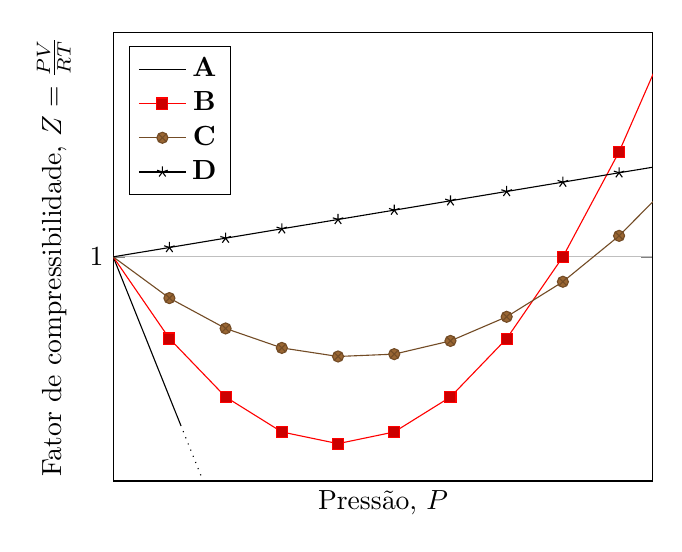
\begin{tikzpicture}
    \begin{axis}
        [
            xlabel = {Pressão, $P$},
            ylabel = {Fator de compressibilidade, $Z = \frac{PV}{RT}$},
            xmin = 0, xmax = 4,
            ymin = -1, ymax = 3,
            xtick = \empty,
            ytick = {1.0}, 
            grid = major,
            legend pos = north west,
        ]
    \addplot [domain = 0:0.5]
        {
            -3*x + 1
        };
    \addplot 
        {
            0.6*(x^2)-2*x+1
        };
    \addplot 
        {
            0.28*(x^2)-1*x+1
        };
    \addplot 
        {
            0.2*x + 1
        };
    \addplot [black, dotted, domain = 0.5:4]
        {
            -3*x + 1
        };
    \legend{\textbf{A},\textbf{B},\textbf{C},\textbf{D}}
    \end{axis}
\end{tikzpicture}